\documentclass[11pt]{article}
%\usepackage{fullpage}
\usepackage{epic}
\usepackage{eepic}
\usepackage{paralist}
\usepackage{graphicx}
\usepackage{tikz}
\usepackage{xcolor,colortbl}

\usepackage{fullpage}
\usepackage{amsmath,amsthm,amssymb}
\usepackage{algorithmicx, algorithm}
\usepackage[noend]{algpseudocode}

\newcommand*\Let[2]{\State #1 $\gets$ #2}
\newtheorem{theorem}{Theorem}
\newtheorem{lemma}[theorem]{Lemma}
\newtheorem{proposition}[theorem]{Proposition}
\newtheorem{corollary}[theorem]{Corollary}

\newenvironment{definition}[1][Definition]{\begin{trivlist}
\item[\hskip \labelsep {\bfseries #1}]}{\end{trivlist}}
\newenvironment{example}[1][Example]{\begin{trivlist}
\item[\hskip \labelsep {\bfseries #1}]}{\end{trivlist}}
\newenvironment{remark}[1][Remark]{\begin{trivlist}
\item[\hskip \labelsep {\bfseries #1}]}{\end{trivlist}}

\newcommand*\Th[1]{{#1}^{\textrm{th}}}

%%%%%%%%%%%%%%%%%%%%%%%%%%%%%%%%%%%%%%%%%%%%%%%%%%%%%%%%%%%%%%%%
% This is FULLPAGE.STY by H.Partl, Version 2 as of 15 Dec 1988.
% Document Style Option to fill the paper just like Plain TeX.

\typeout{Style Option FULLPAGE Version 2 as of 15 Dec 1988}

\topmargin 0pt
\advance \topmargin by -\headheight
\advance \topmargin by -\headsep

\textheight 8.9in

\oddsidemargin 0pt
\evensidemargin \oddsidemargin
\marginparwidth 0.5in

\textwidth 6.5in
%%%%%%%%%%%%%%%%%%%%%%%%%%%%%%%%%%%%%%%%%%%%%%%%%%%%%%%%%%%%%%%%

\pagestyle{empty}
\setlength{\oddsidemargin}{0in}
\setlength{\topmargin}{-0.8in}
\setlength{\textwidth}{6.8in}
\setlength{\textheight}{9.5in}

\setcounter{secnumdepth}{0}

\setlength{\parindent}{0in}
\addtolength{\parskip}{0.2cm}
\setlength{\fboxrule}{.5mm}\setlength{\fboxsep}{1.2mm}
\newlength{\boxlength}\setlength{\boxlength}{\textwidth}
\addtolength{\boxlength}{-4mm}

\newcommand{\algobox}[2]{
  \begin{center}
    \framebox{\parbox{\boxlength}{
        \textbf{Introduction to Algorithms} \hfill \textbf{#1}\\
        \textbf{CS 4820, Spring 2014} \hfill \textbf{#2}}}
  \end{center}}

\newcommand{\algosolutionbox}[2]{
  \begin{center}
    \framebox{\parbox{\boxlength}{
        \textbf{CS 4820, Spring 2014} \hfill \textbf{#1}\\
        #2
      }}
  \end{center}}


\begin{document}

\algosolutionbox{Homework 6, Problem 4}{
  % TODO: fill in your own name, netID, and collaborators
  Name: Piyush Maheshwari\\
  NetID: pm489\\
  Collaborators: None
}

\bigskip

\textbf{(4)}
\emph{(10 points)}
At Ford-Fulkerson University (motto: ``I would find a network whose
maximum flow value is different from its minimum cut capacity, but
there is no such network.'')\ there are many 
committees that need to be staffed with professors.  The 
university has $p$ professors organized into $d$ departments;
each professor belongs to only one department.  There are 
$q$ committees, and the following constraints 
must be satisfied when staffing the committees.
\begin{compactenum}
\item
The required number of professors on committee $k$ is 
specified by a positive integer $r_k$.
\item
No professor is allowed to serve on more than $c$ committees.
\item
No committee is allowed to have more than one professor
from the same department.
\item
For each professor $j$, there is a list $L_j$ of the 
committees on which he or she is qualified to serve.  
Professor $j$ is not allowed to serve on committee $k$
unless $k \in L_j$.
\end{compactenum}
Design a polynomial-time algorithm to determine whether 
it is possible to staff each committee
without violating any of the constraints listed above.
If it is possible to staff the committees, your algorithm should output an
assignment of professors to committees that satisfies
all of the constraints.  The input to the problem
is specified by the numbers $c,d,p,q, r_1,\ldots,r_q$,
and the lists $L_1,\ldots,L_p$.

\bigskip

\subsection{Solution}

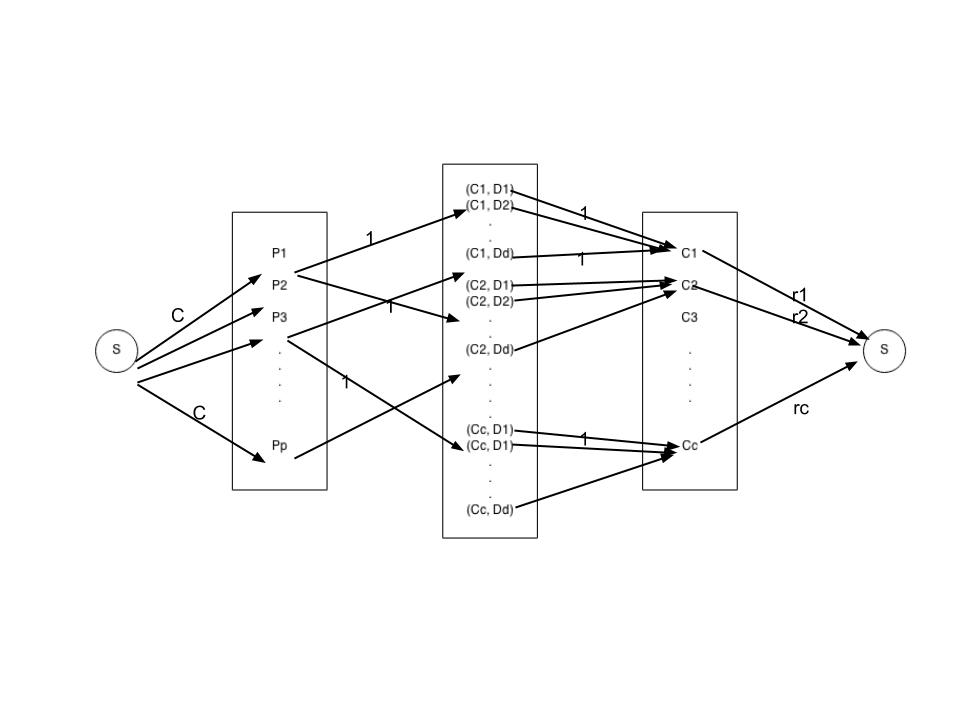
\includegraphics[width=150mm]{flow.jpg}
\newpage
Build a graph G = (V,E) as shown above using steps below.

\begin{enumerate}
\item Add a super source S and super sink T as shown above. Add a vertex $p_i$ for each of the p professors. Add one vertex $(c_i,d_j)$ for every committee c and every department d. The number of such vertexes will be q X d. Then add one vertex $c_i$ for every committee c.
\item Add a edge with capacity c from super source S to every node $p_i$. 
\item Add edge of capacity 1 from vertices $p_k$ to $(c_i,d_j)$ if committee $i$ is in $L_k$ and $p_k$ belongs to department $d_j$.
\item Add edge of capacity 1 from every node $(c_i,d_j)$ to node $c_k$ if $i = k$.
\item Finally add edges of capacity $r_i$ from vertex $c_i$ to super sink $T$
\end{enumerate}

Let $R$ = $\sum\limits_{1}^{q}r_i$	

Now graph G is a flow network with capacity on edges and S and source and T as sink. Now find an integer values max-flow by running Ford-Fulkerson algorithm. If the max-flow value obtained is less then $R$ then an assignment which follows all the constraints is not possible. Otherwise such an assignment is possible. To find the assignment from professors to committees - for each committee vertex $c_i$, find all the edges with nodes $(c_i,d_j)$ to $c_i$ having flow 1. For all such $(c_i,d_j)$ find which $p_k$ are connected to it having flow 1. The set of all such $p_k$'s are assigned to that committee $c_i$. Output the set of assignments for all committees $c_i$'s.
\subsection{Proof of Correctness}

We will show proof correctness by showing a 1-1 correspondence between an integer flow and an assignment. 

First we will show that if there is positive flow on the edge between $p_i$ to $(c_k,d_j)$ from some department $j$ and on the edge between $(c_k,d_j)$ and $c_k$, then professor $p_i$ is part of a committee $c_k$.

Firstly we see that if a professor can only participate in $c$ committees since the inflow on node $p_i$ is c. And since each outgoing edge on $p_i$ is of capacity 1, the outgoing flow cannot exceed c. Then we observe that a vertex $p_i$ is only connected to $(c_k,d_j)$ only if that professor can sit on committee k and is part of the department d. The outgoing flow on every $(c_k,d_j)$ can have a maximum value of 1. This means that there can only be one professor from the department $d_j$ which is part of the committee $c_k$. And since all the edges from $(c_k,d_j)$ go to node $c_k$ and can have maximum flow 1, this means that the inward flow on node $c_k$ will equal to the number of departments from which we have a professor. And since we can only have one professor from one department on a committee, the inflow is also equal to the number of professors sitting on that committee. Finally we observe that the outgoing flow on edges $c_k$ have capacity $r_k$. This means that the outflow cannot exceed $r_k$ which in terms of professor means that there cannot be more than $r_k$ professors on committee $c_k$. 

Since we output a valid assignment only if the flow value is $R$ = $\sum\limits_{1}^{q}r_i$. Note that since the max value on any edge is $r_i$, we can only have this flow if all edges have flow equal to their capacity $r_i$. This will ensure that committee $i$ has exactly $r_i$ professors. 

So by having an integer flow along this path, we satisfy all the constraints of this problem and successfully assign professors to committee. This proves the mapping from integer flow to a valid assignment.


Now we show that if a professor $p_i$ is part of a committee $c_k$, then there must be a positive flow on the edge between $p_i$ to $(c_k,d_j)$ from some department $j$ and on the edge between $(c_k,d_j)$ and $c_k$. If a professor $p_i$ of some department $d_j$ sits on committee $c_k$, then send one unit flow along the edge from vertex $p_i$ to $(c_k,d_j)$. Remaining flow values are forced by flow conservation. Since each committee will have $r_k$ professors, eventually the flow coming out of the vertex $c_k$ will be $r_k$. This proves the mapping from a valid assignment to an integer flow.


This proves the 1-1 correspondence between a valid assignment and an integer flow. Hence if we find such an integer flow with value greater then R, we will have a valid assignment.

\subsection{Running Time}

The graph G will have $O( 2 + p + dq + q)$ vertices. The number of edges will be equal to $O( p + pq + dq + q)$ = $O( q( p + d))$. 
The maximum flow coming out of the sink can be $pc$ since each edge to a $p_i$ can have flow equal to c.

Building the graph takes time equal to $O( V + E)$. We can substitute the value of E and V from above.
We will use the $O(mC)$ bound of FF algorithm. Since this is the slowest step in the algorithm, the running time will be bounded with this. Putting m  = $O( q( p + d))$ and C = $O(pc)$, we have\\\\
Running time = $O(pqc( p + d))$

\end{document}
